\documentclass[tikz,border=7pt]{standalone}
\usepackage{amsmath,amssymb}
\definecolor{cellblue}{RGB}{42,105,168}

\newcommand{\latticeplot}[7]{%
  \begin{scope}[shift={(#1,#2)}]
    \foreach \m in {-1,0,1} {
      \foreach \n in {-1,0,1} {
        \fill[gray!55]
          ({\m*(#3)+\n*(#5)},{\m*(#4)+\n*(#6)}) circle[radius=1.05pt];
      }
    }
    \draw[cellblue,very thick,fill=cellblue!8]
      (0,0)--(#3,#4)--({#3+#5},{#4+#6})--(#5,#6)--cycle;
    \draw[->,cellblue,thick] (0,0)--(#3,#4);
    \draw[->,cellblue,thick] (0,0)--(#5,#6);
    \fill[black] (0,0) circle[radius=1.35pt];
    \node[anchor=north,align=center,text width=4.0cm,font=\small]
      at (0,-3.75) {#7};
  \end{scope}%
}

\begin{document}
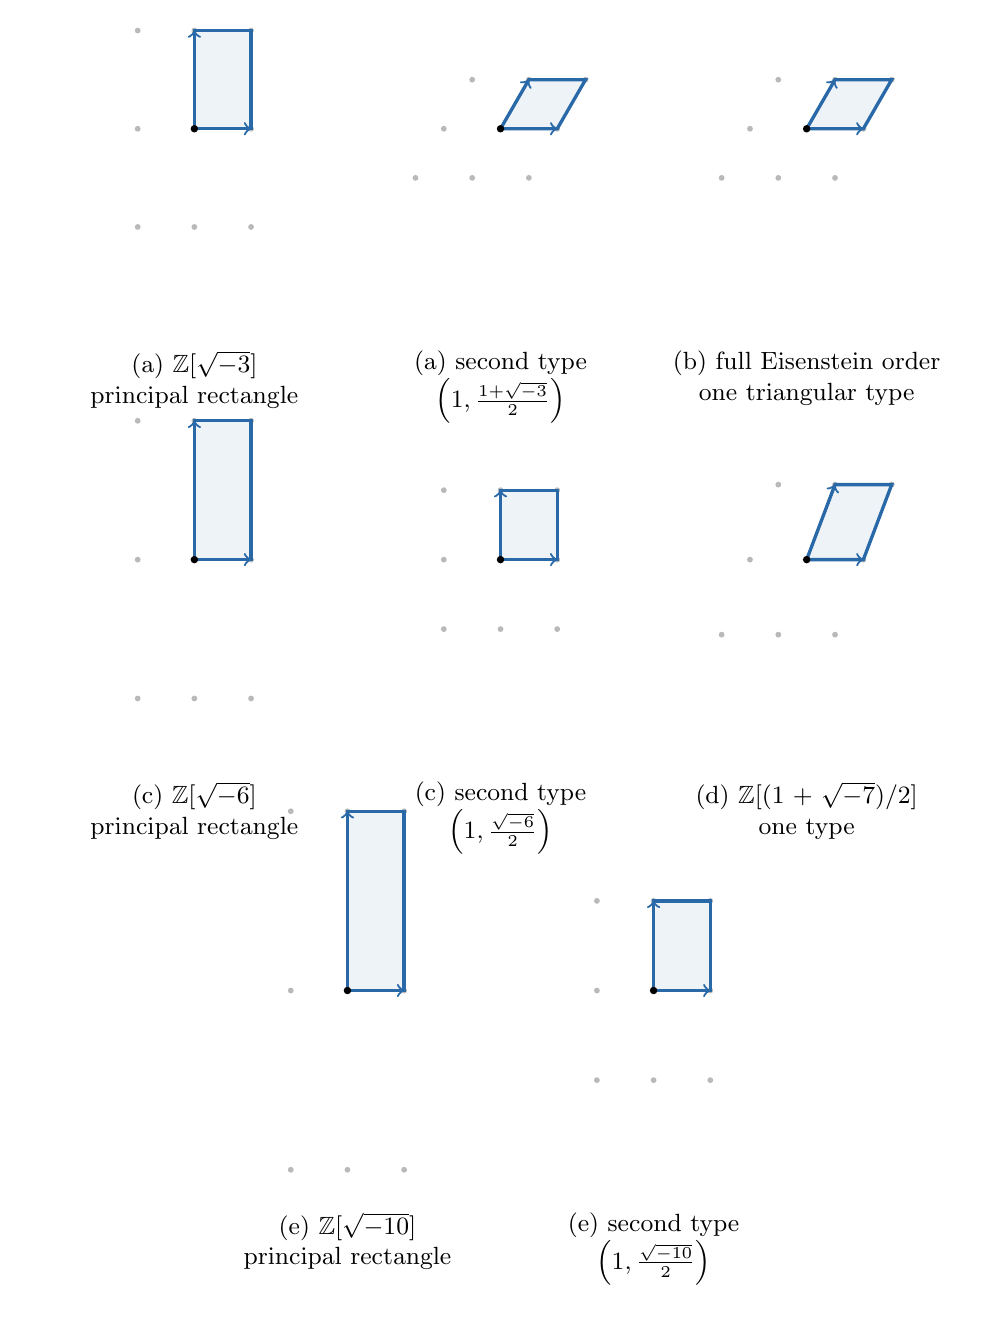
\begin{tikzpicture}[x=0.72cm,y=0.72cm]
  \latticeplot{0}{7.6}{1}{0}{0}{1.732}
    {(a) $\mathbb Z[\sqrt{-3}]$\\principal rectangle}
  \latticeplot{5.4}{7.6}{1}{0}{0.5}{0.866}
    {(a) second type\\$\left(1,\frac{1+\sqrt{-3}}2\right)$}
  \latticeplot{10.8}{7.6}{1}{0}{0.5}{0.866}
    {(b) full Eisenstein order\\one triangular type}

  \latticeplot{0}{0}{1}{0}{0}{2.449}
    {(c) $\mathbb Z[\sqrt{-6}]$\\principal rectangle}
  \latticeplot{5.4}{0}{1}{0}{0}{1.225}
    {(c) second type\\$\left(1,\frac{\sqrt{-6}}2\right)$}
  \latticeplot{10.8}{0}{1}{0}{0.5}{1.323}
    {(d) $\mathbb Z[(1+\sqrt{-7})/2]$\\one type}

  \latticeplot{2.7}{-7.6}{1}{0}{0}{3.162}
    {(e) $\mathbb Z[\sqrt{-10}]$\\principal rectangle}
  \latticeplot{8.1}{-7.6}{1}{0}{0}{1.581}
    {(e) second type\\$\left(1,\frac{\sqrt{-10}}2\right)$}
\end{tikzpicture}
\end{document}
